\documentclass{article}
    \usepackage{multicol}
    \usepackage[heading = true, hyperref]{ctex}
    \ctexset{paragraph/beforeskip=0.5ex, section/beforeskip=1ex, section/afterskip=0.5ex, subsection/beforeskip=1ex, subsection/afterskip=0.5ex, subsubsection/beforeskip=1ex, subsubsection/afterskip=0.5ex}
    \pagestyle{plain}
    \usepackage{geometry}
        \geometry{left=2cm,right=2cm,top=2cm,bottom=2cm}
    \usepackage{amsmath}
    \usepackage{amsfonts}
    \usepackage{siunitx}
    \usepackage{booktabs}
    \usepackage{longtable}
    \usepackage{graphicx}
    \usepackage{subfig}
    \usepackage{float}
    \usepackage{fancyvrb}
    \renewcommand{\labelenumi}{\alph{enumi}.} % Make numbering in the enumerate environment by letter rather than number

    \setlength{\parskip}{0pt}
    \setlength{\parsep}{1ex}
    \linespread{1.1}

    \title{\textbf{基于Caffe深度学习模型的表情视频分类研究} \\ [1.5ex] \begin{large} \emph{结题报告} \end{large} }
    \author{
            张希凡 \\ (2014011103) \\ 清华大学电子工程系无44班 \\ xf-zh14@mails.tsinghua.edu.cn
            \and
            刘本林 \\ (2014011102) \\ 清华大学电子工程系无44班 \\ liubenlin@hotmail.com
            \and
            芦迪 \\ (2014011268) \\ 清华大学电子工程系无41班 \\ me@ludics.cn}
    \date{}

\begin{document}
    \maketitle

\begin{multicols}{2}
    \section{成员及分工}
        \paragraph{张希凡}
        对图像预处理,包括人脸检测、特征点检测与人脸对齐
        \paragraph{芦迪}
        caffe模型设计、训练、测试验证,caffe与matlab接口处理
        \paragraph{刘本林}
        音频特征的提取与处理

    \section{文件清单}
        文件清单如表\ref{tabel:filelist}所示。
        \begin{table*}[htb]
          \centering
          \begin{tabular}{lll}
            \toprule
            \textbf{Directory} & \textbf{File} & \textbf{Description} \\
            \midrule
            /workspace
                        & /fun\_process.m & 视频分类处理函数 \\
                        & /extract.sh & 图像预处理脚本 \\
                        & /model/deploy.prototxt & CaffeNet部署文件 \\
                        & /model/EmotiW.caffemodel & 图像分类模型 \\
                        & /model/faces\_mean.binaryproto & 脸部图像均值文件 \\
                        & /audio/mymfcc.m       & mfcc特征生成函数    \\
                        & /audio/extract\_audio\_feature.m & 音频特征提取函数 \\
                        & /audio/Emotion-from-speech-MFCC-master/  & MFCC第三方实现  \\
                        & /audio/finalNetwork & 音频分类神经网络    \\
                        & /preprocess/face\_landmark\_detection.py & 脸部特征检测脚本 \\
                        & /preprocess/RightPosition\_final & 人脸对齐可执行文件 \\
                        & /preprocess/RightPosition\_final.cpp & 人脸对齐源代码 \\
                        & /preprocess/shape\_predictor\_68\_face\_landmarks.dat & 脸部特征数据 \\
            \midrule
            /report     & /report.pdf & 设计报告(本文档) \\
            \bottomrule
          \end{tabular}
          \caption{文件清单}
          \label{tabel:filelist}
        \end{table*}

    \section{工作开展与完成情况}
        \subsection{基本原理}
            受文献\cite{Fan2016}启发,将视频文件的音频与图像分开处理。对于音频,通过提取音频特征,搭建支持向量机(SVM)模型实现分类。对于图像,则通过深度学习模型实现分类。因为图像背景等因素会对表情分类造成影响,首先进行了预处理。预处理包括人脸检测、特征点检测和人脸对齐。对每个视频文件创建了一个同名文件目录,保存预处理后的脸部图像。将预处理得到的图像分为训练集和测试集,对CaffeNet深度神经网络进行训练,得到了图像分类模型。检测时中和音频与图像的结果。
        \subsection{具体实现}
            \subsubsection{音频特征}
                视频和图片不一样,视频往往会同时带有音频信息。在有些情况下,仅仅通过图像信息是很难对一些视频进行分类,比如并不能截出效果很好的人脸。此时就可以用二者的音频特征缺差异来对视频进行分类。
                \paragraph{特征提取}
                    在音频处理中,最常用的是利用音频的MFCC系数。MFCC是Mel-frequency cepstrum的简称。其使用的是线性的倒频谱表示方法,与人类的非线性听觉 系统更为接近。MFCC得到的是一连串系数,我选用Hamming窗作为窗函数,并在每段时间中取13个MFCC系数以及这13个系数的一阶差分,并求出这26个数在一个视频中的平均值,然后去掉首尾两帧。每个视频得到一个26维的系数向量。

                    其实在最开始的时候,我在特征向量中包含了13个MFCC系数以及其方差、最大值与均值之比和中位数。此外还有最大值、视频能量、过零率以及加窗重采样到的5个点的FFT系数的最大值与方差。然而将这个77维的向量用SVM分类,然而准确率却只有19.6071\%。然后我去掉MFCC系数的方差、最大值与均值之比和中位数,加入了MFCC系数的一阶差分和二阶差分。将新的特征向量送入libsvm,但是分类正确率仅提高了零点几个百分点。
                    但是我将其中多数特征去掉之后,只保留13个MFCC系数以及这13个系数的一阶差分,准确率一下上升到了29.1\%。
                \paragraph{分类器实现}
                    一开始的时候,因为MATLAB自带的SVM只能进行二分类,所以我用的是台湾大学林智仁教授写的libsvm。再采用26维特征后,我发现SVM分类器的交叉验证准确率受参数影响比较大,于是我又采用MATLAB中自带的MATLAB Neural Network Toolbox来完成分类。我用生成的系数矩阵以及label向量训练了一个输入26维,输出为7维,有20个隐含层的神经网络,其具体结构如下图\ref{fig:2}。
                    \begin{figure}[H]
                      \centering
                      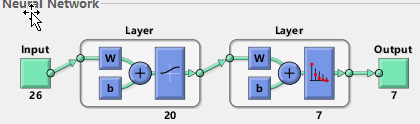
\includegraphics[width=7.4cm]{2.png}
                      \caption{SVM Structure}\label{fig:2}
                    \end{figure}
                    通过对总共765个训练样例随机分类,将其中165个作为测试样例,最后测得准确率能够达到33.7\%,confusion matrix如下图\ref{fig:1}。
                    \begin{figure}[H]
                      \centering
                      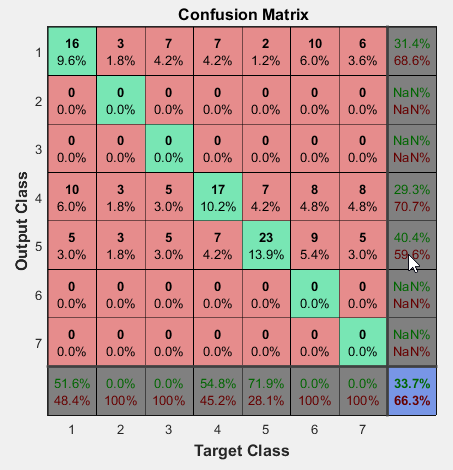
\includegraphics[width=7.4cm]{1.png}
                      \caption{Audio Confusion Matrix}\label{fig:1}
                    \end{figure}
                    可以发现,这个结果其实是过拟合的。输出结果集中在1、4、5三类上。于是我又采用了正则化的手段,但是在将结果平均分布的同时,也大大降低了总正确率,正确率只有不到百分之二十。考虑到过拟合的准确率明显要高出一大截,而且还有图像结果可以依赖,所以音频分类网络的过拟合是可以接受的。
            \subsubsection{图像预处理}
                \paragraph{人脸检测}
                    使用了Dlib库的人脸检测器(Face Detector)。Dlib的人脸检测算法使用了HOG特征、级联分类器、图像金字塔和滑窗检测方案。其中方向梯度直方图(HOG)特征是广泛应用的目标检测的图像特征提取方法。提取图像单元中各像素点的梯度的或边缘的方向直方图,合起来作为特征描述器。这种方法可以很好地描述局部目标的表象和形状。
                    采用这种方法,定位视频每一帧图像的人脸位置,并截出该部分图像。从检测的效果来看,对比之前采用过的OpenCv库中的方法,Dlib库的判别标准较为苛刻,体现在截出的部分基本都对应了图像中的人脸,有个别略微错位,但是检测率较低。Dlib库的人脸检测算法,对正脸的检测效果较好。观察到部分侧脸、一半脸在阴影处的情况,这种算法将无法识别,造成了一部分信息的损失。
                    从视频每帧直接截取的图像,因为人脸朝向、在图像中的位置、面积占比不一,到会对之后网络的训练产生影响。为了消除这种
                    图像间的差异性,避免干扰,考虑进一步对人脸进行对齐。

                \paragraph{特征点检测}
                    进行人脸对齐需要首先获取面部特征点。同样是Dlib库的人脸特征点检测,提供了识别面部68个特征点的方法。该算法实现了文献\cite{jose2014},在iBUG 300-W人脸特征点数据集上进行了训练。这种基于树的人脸关键点检测算法,学习每个关键点的局部二值特征,然后将特征组合起来,使用线性回归检测关键点。每个回归器由很多棵树(tree)组成,每棵树参数是根据 current shape 和 ground truth 的坐标差和随机挑选的像素对训练得到的。
                    这步操作输出68个点对,对应了面部68个特征点,且编号与面部固定的位置相对应(五官、下颌等)。想要将朝向不一的脸对齐,将会利用这些点对,进行位置变换,得到较为统一的人脸形式,作为网络训练的数据。

                \paragraph{人脸对齐}
                    对图像位置变换进行人脸对齐,采用了仿射变换的思想。通过2*3的仿射矩阵,将原坐标(x,y)变为新坐标(x',y')。仿射矩阵的计算依赖于2中检测出的68个点对在原图像中的位置,并为它们设定理想的新坐标,建立之间的映射。调用OpenCv函数计算仿射矩阵,并进行变换,得到对齐后的人脸图像。
                    采用这种方法,相对于具有一定角度的侧脸,对于正脸的处理效果较好。而且采用线性的变换,对于纠正侧向角度较大的样本,比较困难,有其局限性。可以继续考虑采用非线性的变换方式。
                    总的来讲,采用上述方法进行人脸检测和对齐,算法速度较快,且定位精准,是一种较为便利的方法,但是识别率偏低也是一个不足。
            \subsubsection{视觉内容分析}
                采用深度学习方法处理截到的人脸图像。使用的深度神经网络为CaffeNet。因为我们的数据较少,因此使用Caffe官网上下载的bvlc\_reference\_caffenet.caffemodel,采用finetune的方法,对已有的caffemodel进行微调。训练时将前期处理得到的脸部图像分为Train和Val两类,分别进行训练和验证。先将图片数据转化为了Caffe便于读取的lmdb数据库形式,之后对CaffeNet的train\_val.prototxt和solver.prototxt文件进行修改,将输出的数量从1000改为了7。之后开始在服务器上对模型进行训练。

                训练的train loss与accuracy如\ref{fig:4}和\ref{fig:3}所示。
                \begin{figure}[H]
                  \centering
                  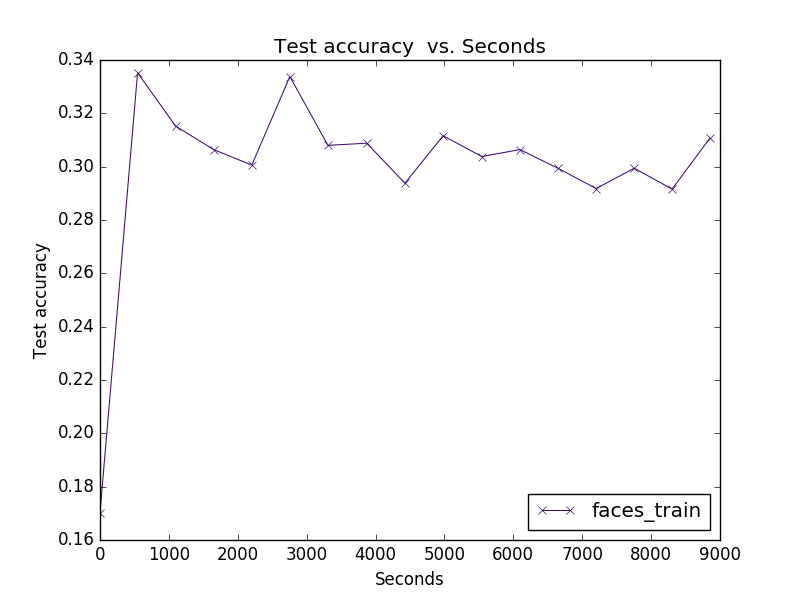
\includegraphics[width=7cm]{test_accuracy.png}
                  \caption{Test Accuracy}\label{fig:3}
                \end{figure}
                \begin{figure}[H]
                  \centering
                  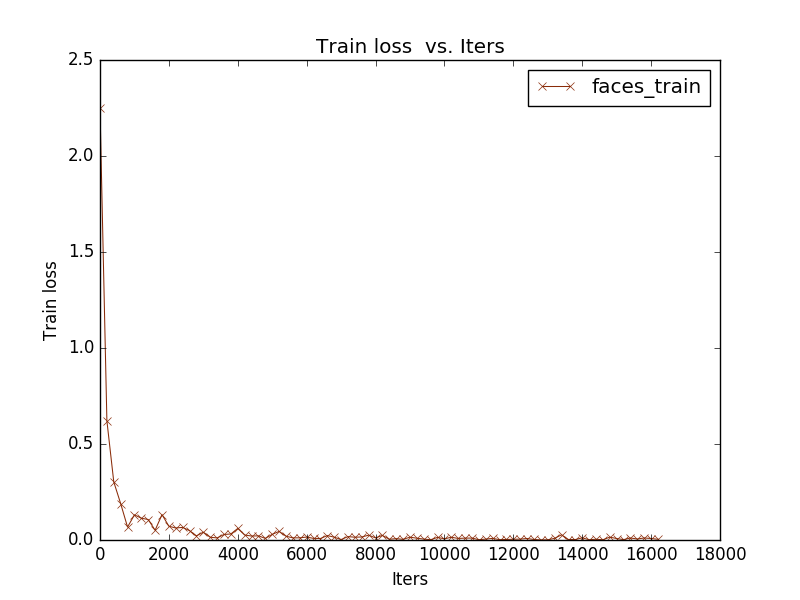
\includegraphics[width=7cm]{train_loss.png}
                  \caption{Train Loss}\label{fig:4}
                \end{figure}

                可以看到Train loss在不断缩小,最终接近于0,证明我们训练的模型收敛了。而Test accuracy则在30\%左右。最终选择使用迭代20000次后的模型。

                对验证集数据基于每个视频进行验证的结果的confusion matrix如图\ref{fig:5}所示。
                \begin{figure}[H]
                  \centering
                  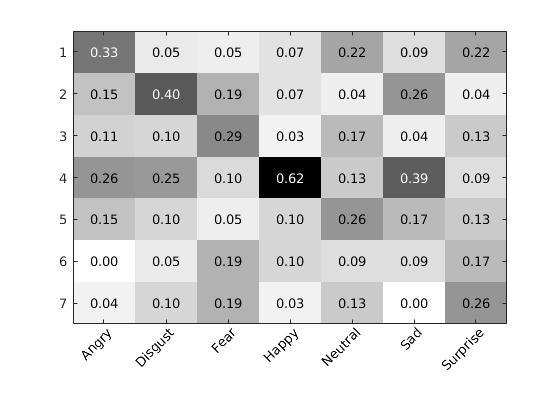
\includegraphics[width=7.4cm]{confusion.jpg}
                  \caption{Image Confusion Matrix}\label{fig:5}
                \end{figure}

                此外,还对AlexNet进行了finetune,但最终的accuracy在27\%左右,且train loss较高,因此最终使用了CaffeNet进行微调后的结果。

        \subsection{问题与不足}
            \paragraph{分类精确度}
            目前分类精确度在不同类别中差异较大,在提高部分我们需要考虑有针对性地予以增强。

            \paragraph{处理速度较慢}
            实现时对音频的处理资源耗费与最终的性能较好,识别速度快,最终的结果也不错。但对图像内容的处理较慢,首先对图像进行预处理,提取每一帧的内容、检测特征点、人脸对齐,耗费的时间较多。提速的方法其实比较简单,因为每个视频只需检测少量的图片,因此以上过程不需要对每一帧都进行处理,但限于时间还没有对这一点进行优化。





    \bibliographystyle{plain}
    \bibliography{ref.bib}

\end{multicols}


\end{document}
